\newpage
\refstepcounter{section}
%Add Image
\vspace*{-40mm} %Make image have no top margin
\begin{tikzpicture}
\node[inner sep=0pt] (x) at (0,0)
    {\hspace{-87mm}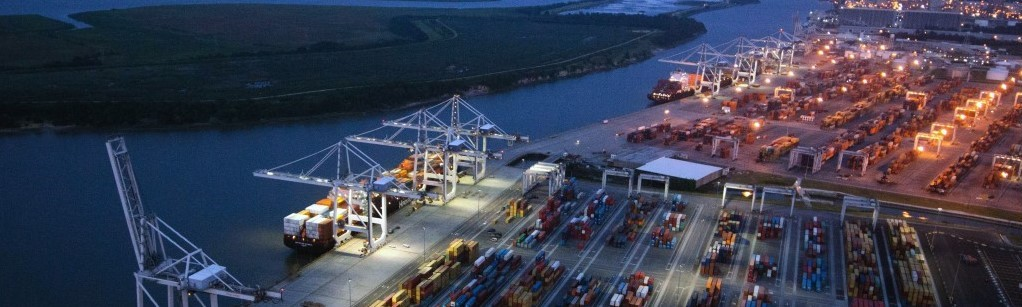
\includegraphics[width=\paperwidth]{sectionimage2.jpg}};
\node[text width=10in] (Z) at (0,-1) {\color{white}\headingfont\Large\bfseries\uppercase{\hspace{-0.7cm}\thesection\hspace{0.5cm}Options}};
\end{tikzpicture}
%Modify TOC
\addcontentsline{toc}{section}{\protect\numberline{\thesection}Options}
  \sectionmark{Options}
\vspace{-2mm}

%Content
\begin{multicols}{2}
\subsection*{Maintain Port of Auckland}
    \subsubsection*{Description}
    \textbf{The first option is to leave the PoA at its current location on reclaimed land in the Waitemata Harbour without development of the Port’s current geography.} \\The Port generates a yearly net profit after tax of approximately \$60 million and facilitates around 187000 jobs. It is comprised of 55ha of wharves and storage areas, the Port can support a 4000 TEU capacity.
    \\Referring to a study of the Port, the Auckland Council planning committee stated in October 2017 that the PoA will not be able to handle long-term freight and cruise demands. With no changes to current procedures, the port is expected to reach maximum capacity by 2030. However, leaving the Port ‘in-situ’ would continue to support the economic centre of freight in New Zealand, provide a best short term economic option in terms of feasibility and maintain the most efficient freight transport to reduce environmental impacts. This will ensure that there is no immediate impact on Auckland's economy and will avoid the need for initial capital investment by taxpayers and the government. It will also ensure that the current income from the port will remain in Auckland and there will be no fluctuation in land returns due to the reallocation of the land for other uses.

    \subsubsection*{Advantages}
    \begin{itemize}[noitemsep]
        \item []\textbf{Financial: }
        \item{If the port is moved, supporting ports will need extensive upgrades. Keeping the port will prevent massive short term costs and excessive revenue losses.}
        \item []\textbf{Natural: }
        \item{Natural resources will be used in upgrading infrastructure should the port be moved.}
        \item []\textbf{Human: }
        \item{Port workers and Auckland based shipping companies will continue to provide economic opportunities for the Auckland region.}
        \item []\textbf{Social: }
        \item{Keeping the port will maintain current jobs in Auckland and will prevent any relocated employees from having to re-settle elsewhere.}
    \end{itemize}
    \subsubsection*{Disadvantages}
    \begin{itemize}[noitemsep]
        \item []\textbf{Financial: }
        \item{Prevents waterfront being used for higher-tech, more profitable real estate (eg to Canary Wharf). Limits diversifying exports/imports in NZ.}
        \item{Restricts economic growth in other areas of NZ.}
        \item []\textbf{Natural: }
        \item{Increased congestion will produce high levels of air and noise pollution}
        \item []\textbf{Human: }
        \item{Prevents new jobs in the region of the new port.}
        \item []\textbf{Social: }
        \item{Congestion will remain significant, which will affect movement of freight in both Auckland and the rest NZ.}
    \end{itemize}



\subsection*{Relocate Port to Northport}

    \subsubsection*{Description}
    \textbf{The second option is to relocate the Port of Auckland and its freight traffic in its entirety to Northport in Marsden Point.}
    \\Northport has the potential to expand their docking length, dry goods storage and develop 180 ha of available industrial land. The draught capability of 13m allows for larger cargo ships, allowing for more cargo transported per litre of fuel consumed. Relocation to Northport will be able to support New Zealand’s increasing freight traffic while simultaneously reducing congestion in Auckland CBD. However, effectively relocating the Port of Auckland to Whangarei would require a major upgrade of the Northland transport system to efficiently distribute freight around the North Island. Currently, there exists a single track North Auckland Line (NAL) which provides freight services between Auckland and Whangarei twice every weekday. Shifting Auckland's freight traffic to aligns well with the current government's plans as the new Labour–NZ First coalition government announced that it would spend \$800 million total on rehabilitating the NAL.

    \subsubsection*{Advantages}
    \begin{itemize}[noitemsep]
        \item []\textbf{Financial: }
        \item{Immediate increase in local jobs available in Whangarei.}
        \item{Immediate decrease in marine traffic in the Auckland Region.}
        \item{Upgrades to the NAL are scheduled by the new coalition government, who could provide significant funding.}
        \item{Increased distribution of Wealth to poorer region (Northland)}
        \item{Constant income of leasing PoA real estate (tourism etc.)}
        \item{The significantly larger port size increases freight capacity.}
        \item{Improvements in the design life of the roads within Auckland. }
        
        
        \item []\textbf{Natural: }
        \item{Reduction in noise pollution in downtown Auckland.}
        \item{Reduced carbon emissions from less fuel usage in cargo ships.}
        
        
        \item []\textbf{Human: }
        \item{Improvement in the aesthetics of downtown Auckland}
        \item{Develop skills in the far north, increase population of working individuals.}
        \item{Decreased congestion in CBD improves the well-being of commuters}
        
        
        \item []\textbf{Social: }
        \item{Improves work ethic and hence socio-economic status of Northland populations.}
        \item{Urban development of the city of Whangarei.}
    \end{itemize}
    \subsubsection*{Disadvantages}
    \begin{itemize}[noitemsep]
        \item []\textbf{Financial: }
        \item{Significant costs of relocation (approx \$5 billion)}
        \item{Heavy cost associated with increasing road and/or capacity (currently 1 lane most of SH1).
        KiwiRail has estimated the cost of getting Northland’s rail network operating to the same standard as other regions as up to \$1 billion, and improving the rail link for freight through Auckland at another \$2 billion to \$3 billion}
        \item []\textbf{Natural: }
        \item{Destruction of habitat to increase roading and/or capacity (SH1)}
        \item []\textbf{Human: }
        \item{Relocation for workers in Port of Auckland}
        \item{Increased congestion between Northland and Auckland.}
        \item []\textbf{Social: }
        \item{Local iwi may be resistant to expansion of Marsden Point Port and Northland Transport network}
    \end{itemize}
 
\subsection*{Relocate Port to Tauranga}
  
    \subsubsection*{Description}
    \textbf{Option 3 is to relocate the PoA and its freight traffic in its entirety to the Port of Tauranga, the most efficient operating port in New Zealand.}
    \\Port of Tauranga currently has two sections in operation at Sulphur Point and Mount Maunganui. With an overall storage capacity available of 22000$m^2$ and with backup land capacity of 90 hectares available, the Port has capacity to grow and develop to meet New Zealand’s future freight demands. The water draught depth of 13.2m, allows the port of Tauranga to accommodate larger ships than the port of Auckland. This reduces the fuel consumption per container shipped. 
    \\The PoT is situated within the ‘Golden Triangle’, bound by Tauranga, Auckland and Hamilton, making it an ideal location for economic growth and distribution of wealth. However, relocation of PoA to Tauranga will require a significant transport infrastructure upgrade of current freight rail network between Auckland and Tauranga. This is to be able to distribute freight efficiently around the North Island and support increased freight traffic capacities from the redirected Auckland freight.  Rail development aligns with the government's plan to update the infrastructure within the ‘golden triangle’ in their Regional Rapid Rail plan.

   \subsubsection*{Advantages}
    \begin{itemize}[noitemsep]
        \item []\textbf{Financial: }
        \item{Tauranga would benefit from the increase in freight traffic from Auckland}
        \item{There's a existing port so one wouldn't have to be built from scratch}
        \item{Pre-existing infrastructure means you wouldn't need to build brand new lines to transport freight}
        \item []\textbf{Natural: }
        \item{Unprocessed industrial land can be developed to increase capacity}
        \item{Reclaimed land previously used for freight can be reallocated for other uses in the CBD}
        \item{reduce shipping based pollution in Auckland harbour}
        \item{Reduction of noise pollution in Auckland CBD}
        \item []\textbf{Human: }
        \item{Increase job opportunities}
        \item{Removal of the PoA will ease traffic congestion}
        \item []\textbf{Social: }
        \item{Further urban development of Tauranga}
        \item{Introduces new areas for the public in the CBD}
        \item{Improves the aesthetic of downtown Auckland}
    \end{itemize}
    \subsubsection*{Disadvantages}
    \begin{itemize}[noitemsep]
        \item []\textbf{Financial: }
        \item{Auckland’s economy would suffer from the delay in shipping (as it is no longer in Auckland)}
        \item{Increased cost of freight between Auckland and Tauranga}
        \item []\textbf{Natural: }
        \item{Increase in ship traffic will contribute to local pollution in Tauranga}
        \item{Expansion of the port will result in the destruction of natural habitats and environments.}
        \item []\textbf{Human: }
        \item{Reduction in job opportunities}
        % \item []\textbf{Social: }
        % \item{Congestion will remain a significant issue, which will affect movement of freight in both the region and the rest of the country.}
    \end{itemize}

\subsection*{Relocate to both Northport \& Tauranga}
    \subsubsection*{Description}
    \textbf{Option 4 is to relocate the waterfront PoA to an inland port and distribute all freight traffic between the Port of Tauranga and Northport. PoA would remain as a cruise ship and ferry docking terminal.}
    \\The relocation enables reclamation of land previously used for the PoA areas to be developed in such a way that it promotes the growth of the region’s tourism revenue. Additionally, this development would also increase the job and upskilling opportunities for those in Northland and Tauranga regions allowing for long-term economic development and increased accessibility for these communities. With the population of Auckland increasing by 50,000 people per year, the demand for freight is higher than ever and cannot be handled by a single operating port. Thus, it is essential to develop ports outside the Auckland region to accommodate the North Island’s inexorable increase in freight traffic. 
    \\Currently, 70\% of imports into the PoA are destined for the Auckland region so effective transport between the centres would be important in maintaining freighting efficiency. However, extensive upgrades to the road and rail network creates exorbitant capital expenses that may be unrealistic. 


    \subsubsection*{Advantages}
    \begin{itemize}[noitemsep]
        \item []\textbf{Financial: }
        \item{Increase in cash flow in Whangarei and Tauranga}
        \item{Population increase in such developing areas.}
        \item []\textbf{Natural: }
        \item{Reduced traffic congestion in Auckland}
        \item{Use of trains to reduce pollution (e.g electric trains)}
        \item []\textbf{Human: }
        \item{Immediate increase in job opportunities}
        \item{Develop skills in Northland and Tauranga}
        \item []\textbf{Social: }
        \item{Use of the waterfront area as a purely as a ‘community’ destination.}
    \end{itemize}
    \subsubsection*{Disadvantages}
    \begin{itemize}[noitemsep]
        \item []\textbf{Financial: }
        \item{The development of rail and road requires large initial investment}
        \item{Requires a large initial investment to establish the increased freight traffic at both ports.}
        \item []\textbf{Natural: }
        \item{Increase in shipping traffic in both harbours}
        \item{Increase in pollution}
        \item []\textbf{Human: }
        \item{Loss of port based jobs in Auckland}
        \item{Lack of these industrial skills in the Auckland region}
        \item []\textbf{Social: }
        \item{Local Iwi at Marsden Point may prevent development of the port and or cause problems in the future with ownership/management}
    \end{itemize}

\subsection*
{Other Ports in Auckland}
    \subsubsection*{Manukau Harbour}
    
        \textbf{Advantages: }{Frees up CBD area, low capital costs as naturally deep}
        \\\textbf{Disadvantages: }{West side(inconvenient), will require constant dredging, a decent population already resides in this area so will not be welcomed at all. Possible conflicts in regards to Mana Whenua and Treaty of Waitangi. Requires a major shift in shipping patterns}
    
    \subsubsection*{Kawakawa Bay}
        \textbf{Advantages: }{Deep water, large draught capacity and requires smaller change in shipping patterns.}
        \\\textbf{Disadvantages: }{Hunua ranges between Kawakawa and Auckland. As there is no existing port there, it must be built from the ground up. Surrounding infrastructure must also be constructed, adding to the overall cost.}
     
    \subsubsection*{Firth of Thames}
        \textbf{Disadvantages: }{Raises environmental, cultural and social issues. Ie: Very nature oriented area of NZ.Large scale reclamation required}
    
    \subsubsection*{Puhinui}
        {\textbf{Advantages: }Highest ranked on their NPV and CBA analysis. Lower capital cost compared to Firth of Thames. Smaller carbon footprint than the currently expanding POA}
        {\\\textbf{Disadvantages: }Will require strict legislations and practices to reduce environmental impacts. Dredging a lot. Future settlements may experience decreased water quality}
    
    \subsubsection*{Muriwai}
        \textbf{Advantages: }{Similar capital costs to making a new port in Firth of Thames.}
        \\\textbf{Disadvantages: }{Far from industrial centres. Further North/West than Manukau. Massive surf and rough weather present difficulties to docking and safety - coastline is exposed to weather from Tasman sea. Terrain inland is full of hills and narrow roads, very difficult to move freight through. Environmental pressure from locals - Large native gannet colony at Muriwai Recreational use of the beaches etc. will be significantly reduced.}  
    
\end{multicols} 

\clearpage